\section{可压缩流体的空气动力学}

\subsection{激波-膨胀波方法}

为了得到升力和阻力($C_L$和$C_D$),可以采用激波-膨胀波方法。

考虑如图所示的具有攻角$\alpha$的菱形机翼。

\begin{figure}[!ht]
    \centering
    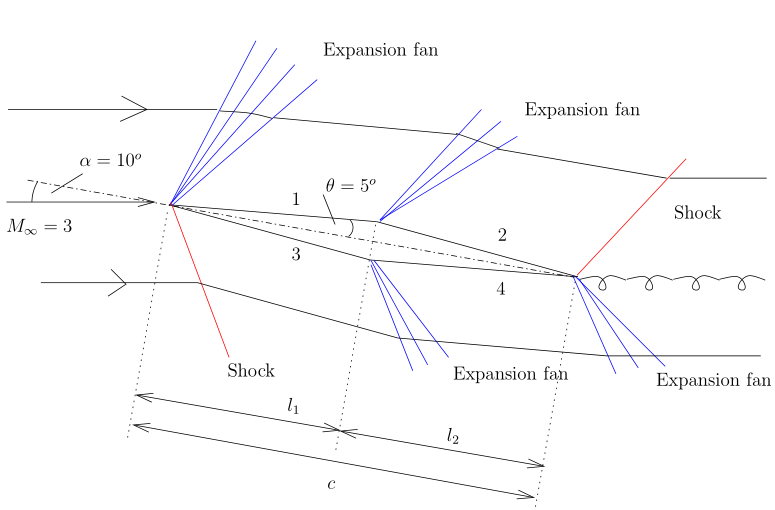
\includegraphics[width=\linewidth]{figures/16.png}
    \caption{菱形机翼示意图}
    \label{16}
\end{figure}

无量纲升力系数$C_L$可以写作

\begin{align*}
    C_L&=\frac{L}{\frac{1}{2}\rho_\infty U_\infty^2 c}\\ 
    &=\frac{L}{\frac{1}{2}a_\infty^2M_\infty^2 c}\\ 
    &=\frac{L}{\frac{1}{2}p_\infty \gamma M_\infty^2c}
\end{align*}

类似地,无量纲阻力系数为

\begin{equation*}
    C_{D}=\frac{D}{\frac{1}{2} p_{\infty} \gamma M_{\infty}^{2} c}
\end{equation*}

要完整的计算升阻力,我们需要各段的压力,求解的方法如下:

\begin{table}[!h]
    \begin{tabular}{cl}
        $M_{\infty} \rightarrow M_{1}$    &   Prandtl-Meyer 关系 \\ 
        $p_{\infty} \rightarrow p_{1}$  &   绝热关系 \\ 
        $M_{1} \rightarrow M_{2}$    &   Prandtl-Meyer 关系 \\ 
        $p_{1} \rightarrow p_{2}$  &   绝热关系 \\ 
        $M_{\infty} \rightarrow M_{3}$    &   激波关系 \\ 
        $p_{\infty} \rightarrow p_{3}$  &   激波关系 \\ 
        $M_{3} \rightarrow M_{4}$    &   Prandtl-Meyer 关系 \\ 
        $p_{3} \rightarrow p_{4}$  &   绝热关系
    \end{tabular}
\end{table}

\subsection{Ackeret理论}

Ackeret理论仅在流体的改变较小、激波相对较弱的情况下成立($\beta\rightarrow\mu$),这也就意味着Ackeret理论只能适用于薄机翼、折射角较小的情况。

利用之前的结论,

\begin{align*}
    \delta \theta&=\pm \frac{\delta p}{\gamma p M^{2}} \sqrt{M^{2}-1}\\ 
    \delta \theta&=\pm \frac{\delta p}{\rho V^{2}} \sqrt{M^{2}-1}
\end{align*}

由于偏折角比较小,我们可以认为$\rho,\ V^2,\ M$均为常数,与来流的状态参数相同($\rho_1,\ V_1^2,\ M_1$。因此,

\begin{equation*}
    \delta \theta=\pm \frac{\delta p}{\rho_{1} V_{1}^{2}} \sqrt{M_{1}^{2}-1}
\end{equation*}

压力系数

\begin{equation*}
    C_p=\frac{p-p_1}{\frac{1}{2}\rho_1V_1^2}
\end{equation*}

由$\delta p=p-p_1$代入前式,可得

\begin{align*}
    \delta \theta&=\frac{C_{p}}{2} \sqrt{M_{1}^{2}-1}\\ 
    C_{p}&=\pm \frac{2 \delta \theta}{\sqrt{M_{1}^{2}-1}}
\end{align*}

考虑上式的$\delta\theta$为一个微小的角度$\eta$,则有

\begin{equation*}
    \pm C_{p}=\frac{2 \eta}{\sqrt{M_{\infty}^{2}-1}}
\end{equation*}

取正号时代表机翼的上表面,取负号时代表机翼的下表面。再次强调,基于Ackeret理论的分析只适用于攻角小、机翼薄的情形。

考虑一片任意的机翼,他都可以被分解为三个元素的叠加:攻角$\alpha$的弦线,厚度分布(两侧对称)$t(x)$,以及弯度分布(两侧不对称)$\xi(t)$,如图\ref{14}所示。

\begin{figure}[!ht]
    \centering
    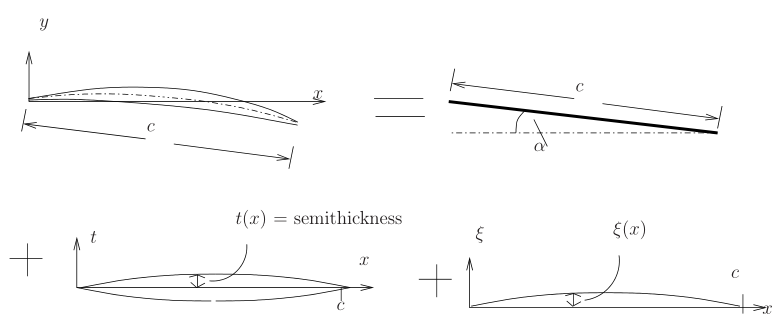
\includegraphics[width=\linewidth]{figures/17.png}
    \caption{机翼的分解}
    \label{17}
\end{figure}

先前讨论的$\eta$为转角,因此$\eta=dy/dx$,对于上下表面各有:

\begin{align*}
    \left(\frac{d y}{d x}\right)_{U}&=-\alpha+\frac{d t(x)}{d x}+\frac{d \xi(x)}{d x}\\ 
    \left(\frac{d y}{d x}\right)_{L}&=-\alpha-\frac{d t(x)}{d x}+\frac{d \xi(x)}{d x}
\end{align*}

\textbf{上表面}

\begin{figure}[!ht]
    \centering
    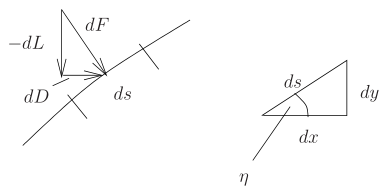
\includegraphics[width=8cm]{figures/18.png}
    \caption{上表面受力}
    \label{18}
\end{figure}

如图\ref{18},取微元,则该微元的守力为

\begin{equation*}
    d F=p d s
\end{equation*}

代入$C_p$,可以得到

\begin{align*}
    p&=C_{p} \frac{1}{2} \rho_{\infty} U_{\infty}^{2}+p_{\infty}\\ 
    d F&=C_{p_{U}} \frac{1}{2} \gamma p_{\infty} M_{\infty}^{2} d s+p_{\infty} d s
\end{align*}

升力:

\begin{align*}
    d L&=-C_{p_{U}} \frac{1}{2} \gamma p_{\infty} M_{\infty}^{2} \cos \eta d s-p_{\infty} \cos \eta d s\\ 
    &=-C_{p_{U}} \frac{1}{2} \gamma p_{\infty} M_{\infty}^{2} d x-p_{\infty} d x
\end{align*}

阻力:

\begin{align*}
    d D&=C_{p_{U}} \frac{1}{2} \gamma p_{\infty} M_{\infty}^{2} \sin \eta d s+p_{\infty} \sin \eta d s\\ 
    &=C_{p_{U}} \frac{1}{2} \gamma p_{\infty} M_{\infty}^{2} d y+p_{\infty} d y\\ 
    &=C_{p_{U}} \frac{1}{2} \gamma p_{\infty} M_{\infty}^{2}\left(\frac{d y}{d x}\right)_{U} d x+p_{\infty}\left(\frac{d y}{d x}\right)_{U} d x
\end{align*}

\textbf{下表面}

如图\ref{19},类似地可以得到

\begin{figure}[!ht]
    \centering
    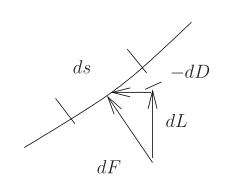
\includegraphics[width=8cm]{figures/19.png}
    \caption{下表面受力}
    \label{19}
\end{figure}

\begin{align*}
    d L&=C_{p_{L}} \frac{1}{2} \gamma p_{\infty} M_{\infty}^{2} d x+p_{\infty} d x\\ 
    d D&=-C_{p_{L}} \frac{1}{2} \gamma p_{\infty} M_{\infty}^{2}\left(\frac{d y}{d x}\right)_{L} d x-p_{\infty}\left(\frac{d y}{d x}\right)_{L} d x
\end{align*}

\textbf{总升力与总阻力}

对$dL$和$dD$积分,并近似$\cos\alpha\approx 1$,

\begin{align*}
    L&=\frac{1}{2} \gamma p_{\infty} M_{\infty}^{2} \int_{0}^{c}\left(C_{p_{L}}-C_{p_{U}}\right) d x\\ 
    D&=\frac{1}{2} \gamma p_{\infty} M_{\infty}^{2} \int_{0}^{c}\left[C_{p_{U}}\left(\frac{d y}{d x}\right)_{U}-C_{p_{L}}\left(\frac{d y}{d x}\right)_{L}+p_{\infty}\left\{\left(\frac{d y}{d x}\right)_{U}-\left(\frac{d y}{d x}\right)_{L}\right\}\right] d x
\end{align*}

代入${C_P}_U$,${C_P}_L$,以及$\eta_U$,$\eta_L$

\begin{equation*}
    L=\frac{-\gamma p_{\infty} M_{\infty}^{2}}{\sqrt{M_{\infty}^{2}-1}}\left[\int_{0}^{c}(-2 \alpha) d x+\int_{0}^{c}\left(\frac{d t}{d x}+\frac{d \xi}{d x}\right)_{U} d x-\int_{0}^{c}\left(\frac{d t}{d x}-\frac{d \xi}{d x}\right)_{L} d x\right]
\end{equation*}

不难看出,

\begin{equation*}
    \int_{0}^{c}\left(\frac{d t}{d x}+\frac{d \xi}{d x}\right) d x=0
\end{equation*}

可以得到

\begin{equation*}
    L=\frac{\gamma p_{\infty} M_{\infty}^{2} 2 \alpha c}{\sqrt{M_{\infty}^{2}-1}}
\end{equation*}

\begin{align*}
    C_{L}&=\frac{L}{\frac{1}{2} \rho_{\infty} U_{\infty}^{2} c}=\frac{L}{\frac{1}{2} \gamma p_{\infty} M_{\infty}^{2} c}\\ 
    &=\frac{4 \alpha}{\sqrt{M_{\infty}^{2}-1}}
\end{align*}

我们可以得到,升力系数与$\alpha$成正比,并且不依赖于机翼形状。实验证明,Ackeret理论在马赫数$M>1.5$,攻角$\alpha<8^\circ$时是相对准确的。

类似地,可以得到阻力

\begin{equation*}
    D=\frac{2 \gamma p_{\infty} M_{\infty}^{2}}{\sqrt{M_{\infty}^{2}-1}} \int_{0}^{c}\left\{\alpha^{2}+\left(\frac{d t}{d x}\right)^{2}+\left(\frac{d \xi}{d x}\right)^{2}\right\} d x
\end{equation*}

定义

\begin{align*}
    \overline{\left(\frac{d t}{d x}\right)^{2}}&=\frac{1}{c} \int_{0}^{c}\left(\frac{d t}{d x}\right)^{2} d x\\ 
    \overline{\left(\frac{d \xi}{d x}\right)^{2}}=\frac{1}{c} \int_{0}^{c}\left(\frac{d \xi}{d x}\right)^{2} d x
\end{align*}

可得

\begin{equation*}
    D=\frac{2 \gamma p_{\infty} M_{\infty}^{2}}{\sqrt{M_{\infty}^{2}-1}}\left\{\alpha^{2}+\overline{\left(\frac{d t}{d x}\right)^{2}} c+\left(\frac{d \xi}{d x}\right)^{2} c\right\}
\end{equation*}

\begin{equation*}
    C_{D}=\frac{4}{\sqrt{M_{\infty}^{2}-1}}\left\{\alpha^{2}+\overline{\left(\frac{d t}{d x}\right)^{2}}+\overline{\left(\frac{d \xi}{d x}\right)^{2}}\right\}
\end{equation*}

由上式可以知道,阻力系数不仅依赖于攻角$\alpha$,同样也和机翼形状有关。

喷管出口的流体也可以应用Ackeret理论,

$p_1>p_0$,则如图\ref{20}所示;$p_1<p_0$,则如图\ref{21}所示。

\begin{figure}[!htb]
    \centering
    \subfigure[$p_1>p_0$]{
    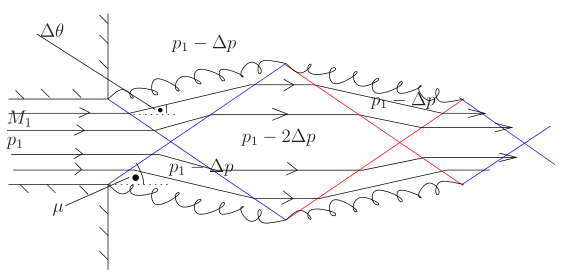
\includegraphics[width=0.4\linewidth]{figures/20.png}
    \label{20}
    }
    \quad
    \subfigure[$p_1<p_0$]{
    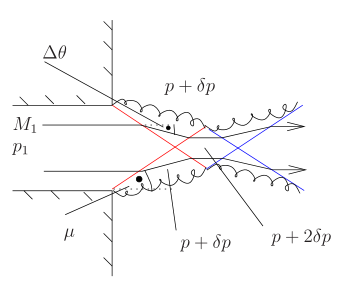
\includegraphics[width=0.4\linewidth]{figures/21.png}
    \label{21}
    }
    \caption{喷管出口的流体}
\end{figure}



